\documentclass[DM,authoryear,toc]{lsstdoc}
% lsstdoc documentation: https://lsst-texmf.lsst.io/lsstdoc.html
\input{meta}

% Package imports go here.
\usepackage[alsoload=hep]{siunitx}

% Local commands go here.

%If you want glossaries
%\input{aglossary.tex}
%\makeglossaries

\title{Seeing values for LSST strategy simulations}

% Optional subtitle
% \setDocSubtitle{A subtitle}

\author{%
Eric Neilsen
}

\setDocRef{RTN-022}
\setDocUpstreamLocation{\url{https://github.com/lsst/rtn-022}}

\date{\vcsDate}

% Optional: name of the document's curator
% \setDocCurator{The Curator of this Document}

\setDocAbstract{%
The \texttt{opsim4} operations simulation program for the LSST astronomical survey uses a database of seeing values covering the range of times to be simulated. I describe the creation of such a database using Dual Image Motion Monitor (DIMM) data collected at Cerro Pachon from 2004-03-17 to 2019-10-07. In times during which the data overlap, I compare the distribution of DIMM seeing values to the seeing measured in DECam images, taken at a site ~10 km away. Because instrumental problems in the DIMM may indicate unreliable measurements, cuts on image quality (as indicated by the measured Strehl ratio) were explored. The DIMM has significant gaps, so I model the data (with and without cuts on Strehl ratio) and generate artificial data in the gaps according to the model. The model consists of a sinusoidal variation with a period of one year, an autoregressive (AR1) model for variations in mean seeing from one night to the next, and another AR1 model for variations on a 5 minute timescale. I create four databases according to this procedure, two based on DIMM data starting 2006-01-01 (with and without a Strehl ratio cut), and two starting 2009-01-01. I then run \texttt{opsim} simulations using each, and an otherwise identical simulation using the default seeing database, and explore the differences.
}

% Change history defined here.
% Order: oldest first.
% Fields: VERSION, DATE, DESCRIPTION, OWNER NAME.
% See LPM-51 for version number policy.
\setDocChangeRecord{%
  \addtohist{2}{2022-03-04}{Published}{Eric Neilsen}
  \addtohist{1}{2021-06-23}{Documentation draft}{Eric Neilsen}
}


\begin{document}

% Create the title page.
\maketitle
% Frequently for a technote we do not want a title page  uncomment this to remove the title page and changelog.
% use \mkshorttitle to remove the extra pages

% ADD CONTENT HERE
% You can also use the \input command to include several content files.


\section{Introduction}
\label{sec:intro}

The Vera C. Rubin Observatory is currently under construction on Cerro
Pachon, in Chile. It will spend 10 years performing Legacy Survey of
Space and Time (LSST), taking repeated images across a large fraction
of the sky visible from Cerro Pachon.

Turbulence in the Earth's atmosphere causes short time-scale variations
in the index of refraction of the air. These variations place limits
on the sharpness of astronomical images taken by telescopes on the
surface of the Earth; this limit is called the ``seeing'', typically
measured as the angular full width at half maximum (FWHM) of the image
of a point source, the ``point spread function'' (PSF), that would be
taken by an ideal instrument. The seeing is a property of the weather,
and as such is correlated with the location, time of year, and
transient weather patterns. \cite{2009PASP..121..922E}, for example,
measure a significant variation in seeing with time of year at Cerro
Tololo, a site $\sim10 \mbox{ km}$ from Cerro Pachon.

The \texttt{opsim} operations simulation follows candidate survey
strategies to generate a database of exposures plausible for an
execution of the survey. Each exposure in the database includes
several parameters, including the time the exposure was taken, the
depth of the image (the brightness of the faintest objects detected at
a given signal to noise ratio), and the delivered PSF FWHM. The LSST
project and science groups use these databases to evaluate the
different operations strategies. Such evaluations can then be used
both to select among candidate observing strategies, and set
expectations for the scientific usefulness of the LSST data set.

To calculate the depth and PSF FWHM of each simulated exposure, the
simulator must have a value for the atmospheric seeing at the time the
image was taken. It takes these values from a simple database table, which
provides atmospheric seeing values at a set of times.

The details of the seeing database used by \texttt{opsim}
can affect the results in several ways:

\begin{itemize}
  \item The global quality of the survey is strongly affected by the
    contents of the seeing database. If the average seeing in the
    seeing database is worse, the average delivered PSF FWHM in the
    images that comprise the survey will be worse, as will the depth
    of the survey.
  \item The accessible area in the sky varies with a period of one
    year, which corresponds to the yearly seasonal variation in the
    seeing. For example, the same area on the sky can be imaged in
    January every year, and a different area every July. If the seeing
    is better in January than in July of every year, then the data
    quality in the area of sky accessible in January will be better
    than that accessible in July.
  \item The autocorrelation of seeing over time will also affect the
    data quality of light curves of transient objects: if the seeing
    is weakly correlated over timescale similar to the duration of a
    transient event, then the quality of different points on the light
    curve will be uncorrelated. On the other hand, if the
    autocorrelation of the seeing over time is strong on the timescale
    of the event, then it is more likely for the seeing to be either
    good or poor over the whole duration of the event.
  \item The autocorrelation of the seeing over time on timescales
    similar to the time between one exposure and the next will affect
    the ability of the scheduler to react appropriately to changes in
    seeing, if the strategy calls for it to do so.
    
\end{itemize}

The seeing conditions on Cerro Pachon have been monitored since 2004
using a Dual Image Motion Monitor, or DIMM. A DIMM measures the
position of a star through two neighboring paths through the
atmosphere, typically separated by $\sim10 \mbox{ cm}$. The difference
in positions between these two paths indicates the variability in
measured position due to turbulence on that spatial scale. The Fried
parameter, the diameter of a circular aperture over which the RMS
wavefront error induced by atmospheric turbulence is one radian, can
be derived directly from DIMM measurements [\cite{1965JOSA...55.1427F,
    1987PASP...99.1360M, 2002PASP..114.1156T}].

The archive of DIMM data for Cerro Pachon records seeing values
derived for $500\nm$ light using a Kolmogorov turbulence model,
which may be pessimistic. \cite{2002PASP..114.1156T} provides a
formula for approximating a more realistic von K\'arm\'an model,
provided one can estimate the outer scale of the turbulence.

The default seeing database used by \texttt{opsim4} version 081217 was
artificially generated from a model derived from a limited set of
data from the Cerro Pachon DIMM, and repeats with a period of two
years.

Observing strategy simulation for the Dark Energy Survey (DES)
[\cite{2016MNRAS.460.1270D}] had a similar
requirement. \texttt{obstac} [\cite{2014ASPC..485...77N}], the DES operations
scheduler and simulator, used seeing data sets generated using a model
derived from data from the DIMMs on Cerro
Tololo [\cite{2012ASPC..461..201N}]. The model used by \texttt{obstac} included
both a seasonal component and a short timescale autoregressive model,
producing seeing values on 5 minute intervals.

%% Plots in this note were generated using \texttt{jupyter} notebooks
%% that can be found in github:
%% \url{https://github.com/LSSTDESC/obs_strat/tree/master/doc/seeing}. The
%% \texttt{simsee} application itself can be found in the same product:
%% \url{https://github.com/LSSTDESC/obs_strat/tree/master/code/simsee}. Data
%% files not included in the \texttt{github} product can be found in the
%% \texttt{/global/project/projectdirs/lsst/survey\_sims/input/seeing}
%% directory on \texttt{cori.nersc.gov}.

% ----------------------------------------------------------------------

\section{Overview}
\label{sec:overview}

The following procedure was followed in generating new seeing
databases and exploring their effects on \texttt{opsim4} simulations:

\begin{itemize}

  \item Obtain the Cerro Pachon DIMM data and explore it
    interactively, as provided. See section~\ref{sec:dimm}.
  \item Validate the DIMM data through comparison with seeing
    estimated using DECam and Gemini South imaging. Examine the
    agreement between these data sets as a function of the Strehl
    ratio recorded for the DIMM, and filter the DIMM data accordingly
    (if necessary).
  \item For each DIMM measurement, calculate the Fried parameter,
    $r_{0}$, and seeing based on the von K\'arm\'an model using the
    correction given in \cite{2002PASP..114.1156T} and an outer scale
    of $\mathcal{L}_{0} = 30$ meters, based on the measurement
    reported in \cite{2000ApOpt..39.5415Z}.
  \item Resample the DIMM data to obtain a data set sampled on 5
    minute intervals.
  \item Create two seeing data sets for LSST observing nights by
    shifting the resampled DIMM data by 4748 nights (13 years) or 5844
    nights (16 years), and filling in the gaps in DIMM data using
    random data according to a time series model derived from the DIMM
    data.
  \item Create two additional seeing data sets for LSST observing
    nights by filtering the resampled DIMM data to remove data with
    suspiciously low Strehl ratios, then shifting and filling in the
    filtered data following the same procedure applied to unfiltered
    data.
  \item Run five \texttt{opsim4} simulations: one using the default seeing
    database, and one for each of the newly generates seeing
    databases, and compare the results.
\end{itemize}

The following procedure produced the model used to generate artificial seeing values for times corresponding to gaps in DIMM data:

\begin{itemize}
  \item Interactively explore long time-scale variability, and fit a
    sine with a period of 1 year to the nightly mean value of
    $\log(r_{0})$.
  \item Interactively explore the nightly residuals of $\log(r_{0})$
    (after subtraction of the seasonal model), and fit the residuals
    using autoregressive (AR1) models on each uninterrupted sequence
    of consecutive nights with DIMM data. Derive a global AR1 model
    for nightly residuals using a weighted average of the parameters
    as derived from each sequence of nights.
  \item Interactively explore the short time-scale residuals of
    $\log(r_{0})$ (after subtraction of the nightly mean values), and
    fit the residuals using a second autoregressive (AR1) model on
    each consecutive sequence of values in the resampled data. (Gaps
    in DIMM data during the night result in breaks between sequences
    in the resampled data.) Derive a global AR1 model for short
    time-scale residuals using a weighted average of the parameters as
    derived from each sequence.
\end{itemize}


\section{Cerro Pachon DIMM data}
\label{sec:dimm}

\cite{ebustos} kindly provided Cerro Pachon DIMM data in the
form of two text tables, each with a timestamp and an
airmass-corrected seeing value for a wavelength of $500\nm$,
derived using a Kolmogorov seeing model.

Figures~\ref{fig:decam-monthly-dimm-vs-year}
and~\ref{fig:gemini-monthly-dimm-vs-year} show the variation in
reported FWHM seeing values with time. The regular extremes of good
and poor seeing, shortly after the start and midpoint of each year,
match well with anecdotal experience, and indicate a significant
seasonal component. There are also noticeable long-term trends, but on
a timescale comparable to or greater than the range of the data, so no
attempt is made to model these longer-term trends here. This feature
is also evident in the autocorrelation function of the nightly means.

\begin{figure*}
  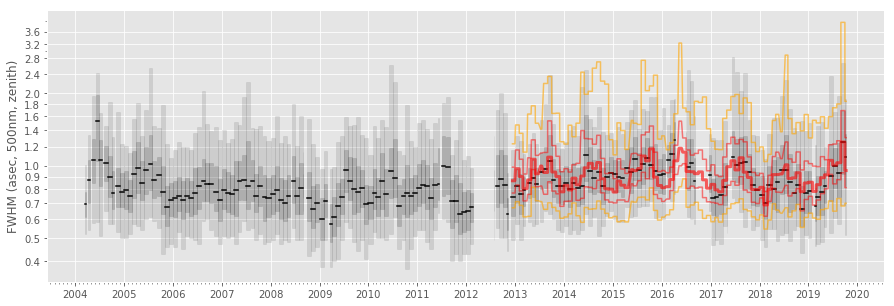
\includegraphics[width=\columnwidth]{./figures/monthly_dimm_vs_year.png}
  \caption{
    Horizontal black lines show the median (Kolmogorov) DIMM seeing in each
    month. Dark gray bars extend from the first through the third
    quartiles for each month, and light bars from the 5\% to 95\%
    quantiles.    
    The thick red line shows the median FWHM seeing as derived from
    DECam imaging (after subtraction in quadrature of a 0.45''
    instrumental contribution, and correction to zenith and
    500nm). Thin red lines show the first and third quartiles, and
    thin orange lines, the 5\% and 95\% quantiles.
    }
  \label{fig:decam-monthly-dimm-vs-year}
\end{figure*}

\begin{figure*}
  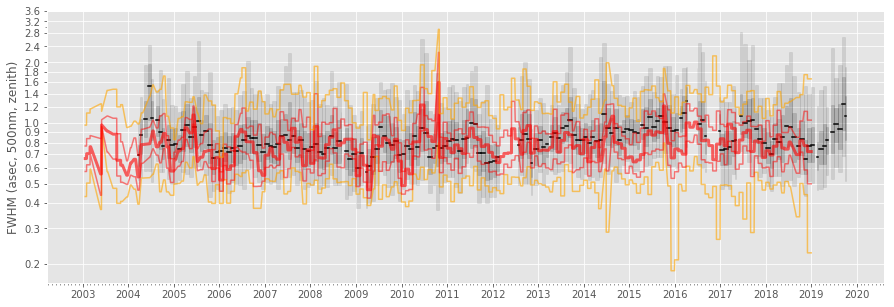
\includegraphics[width=\columnwidth]{./figures/monthly_gemini_dimm_vs_year.png}
  \caption{
    Horizontal black lines show the median (von K\'arm\'an,
    $\mathcal{L}_{0} = 30$m) DIMM seeing in each month. Dark gray bars
    extend from the first though the third quartiles for each month,
    and light bars from the 5\% to 95\% quantiles.
    The think red line shows the median FWHM seeing as derived from
    Gemini South IQ data. Thin red lines show the first and third
    quartiles, and thin orange lines the 5\% and 95\% quantiles.  }
  \label{fig:gemini-monthly-dimm-vs-year}
\end{figure*}



%% Figure~\ref{fig:dimm-vs-decam} compares the seeing quantiles for
%% different months of DIMM and DECam data. The correspondence is worst
%% when the seeing is very poor (and so is unlikely to be useful in any
%% case), and in very good seeing, during which DECam seems to hit a hard
%% floor (about where the PSF becomes undersampled).

%% \begin{figure*}
%%   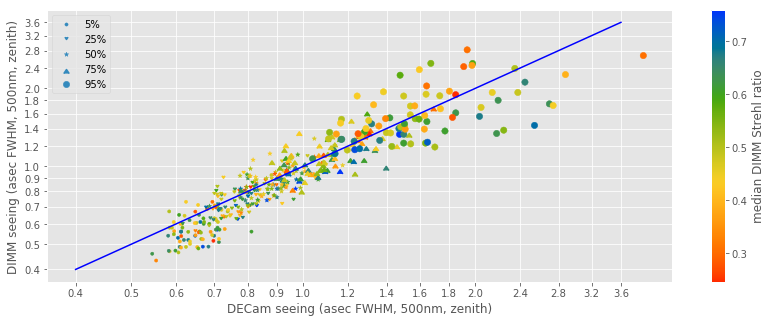
\includegraphics[width=\columnwidth]{./figures/dimm_vs_decam.png}
%%   \caption{
%%     Each point represents a quantile in the FWHM distribution of a
%%     month, as measured by DECam (horizontal axis) and the DIMM
%%     (vertical). The shape and size indicated which quantile, and the
%%     color the median DIMM Strehl ratio in that month.
%%     }
%%   \label{fig:dimm-vs-decam}
%% \end{figure*}

Figure~\ref{fig:gemini-vs-dimm} plots monthly quantiles of DIMM seeing
against corresponding quantiles of Gemini South IQ data. If the
monthly distributions matched, all points would fall on the blue line.
The correspondence is worst when the seeing is very poor (and so is
unlikely to be useful in any
case). Figure~\ref{fig:gemini-vs-dimm-hexbin} compares corresponding
hourly means, and shows a similarly close correspondence.

\begin{figure*}
  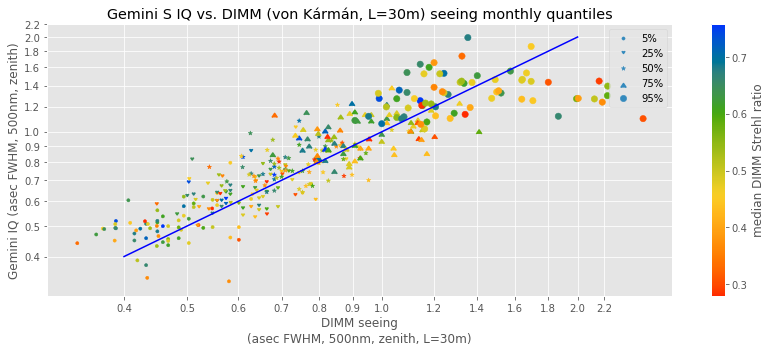
\includegraphics[width=\columnwidth]{./figures/geminiIQ_vs_dimm.png}
  \caption{
    Each point represents a quantile in the FWHM distribution of a
    month, as measured by the DIMM (horizontal axis) and Gemini South IQ
    (vertical). The shape and size indicated which quantile, and the
    color the median DIMM Strehl ratio in that month.
    }
  \label{fig:gemini-vs-dimm}
\end{figure*}

\begin{figure*}
  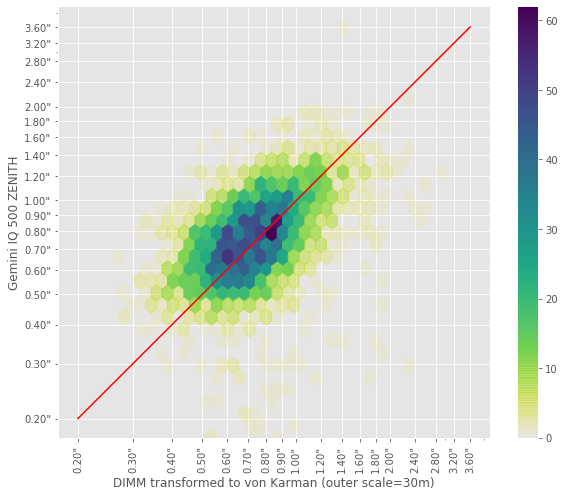
\includegraphics[width=\columnwidth]{./figures/geminiIQ_vs_dimm_hexbin.png}
  \caption{ Color represents counts of hours in hexagonal bins in
    Gemini IQ vs DIMM seeing space. The red line shows a perfect
    match. Except for seeing values better than 0.4'', DIMM values
    predict the Gemini IQ values well, on average.}
  \label{fig:gemini-vs-dimm-hexbin}
\end{figure*}


\section{DIMM data quality and Strehl ratio}

The legacy seeing database used by \texttt{opsim} (current as of
October 2019) uses a seeing database artificially generated using
statistics derived from Pachon DIMM data taken between 2004-05-06 and
2006-01-20. These statistics were derived from the DIMM data after the
application of a cut on the Strehl ratio of the left star in the DIMM
images, because this might be an indication that the DIMM is out of
focus or misaligned, and therefore providing unreliable results. (See
Wang et al. 2006.) Figure~\ref{fig:claver-strehl-cut} shows the data used to
generate this database. The sharp cutoff in Strehl ratios indicates
that the cut value was 0.3 for data taken before 2005-06-17
(MJD=53538), and 0.5 for data taken after.

\begin{figure*}
  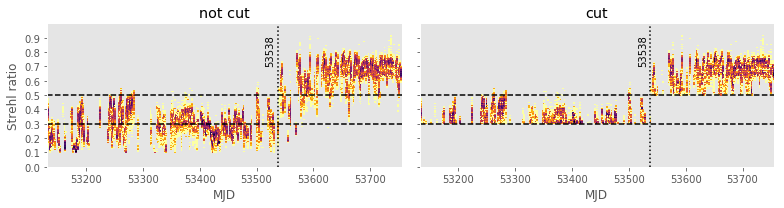
\includegraphics[width=\columnwidth]{./figures/claver_strehl_cut.png}
  \caption{
    2D histograms of the left DIMM Strehl ratio and date in the subset
    of DIMM data used to generate the legacy \texttt{opsim} seeing data, before
    (left) and after (right) application of cuts on Strehl ratios.
  }
  \label{fig:claver-strehl-cut}
\end{figure*}

A low Strehl ratio is not necessarily an indication of poor DIMM data
quality, however: it may also be low due to atmospheric seeing
itself. Figure~\ref{fig:strehl-boxplots} shows both of these effects:
the upper panel shows that DIMM and Gemini South seeing are well-matched except when the Strehl ratio falls below 0.15, where the DIMM
shows wider PSF FWHMs than the corresponding Gemini data. On the other
hand, the lower panel shows that the DECam seeing is genuinely worse
when the DIMM Strehl ratio is less than 0.25, such that filtering the
DIMM data based on Strehl ratio will bias the data in the other
direction. Fortunately, the fraction of DIMM data with a Strehl ratio
below 0.15 is low (see figure~\ref{fig:strehl-hist}), so any effect
will be minor. Seeing simulations based on cut and uncut DIMM data
will be used to indicated the range.

\begin{figure*}
  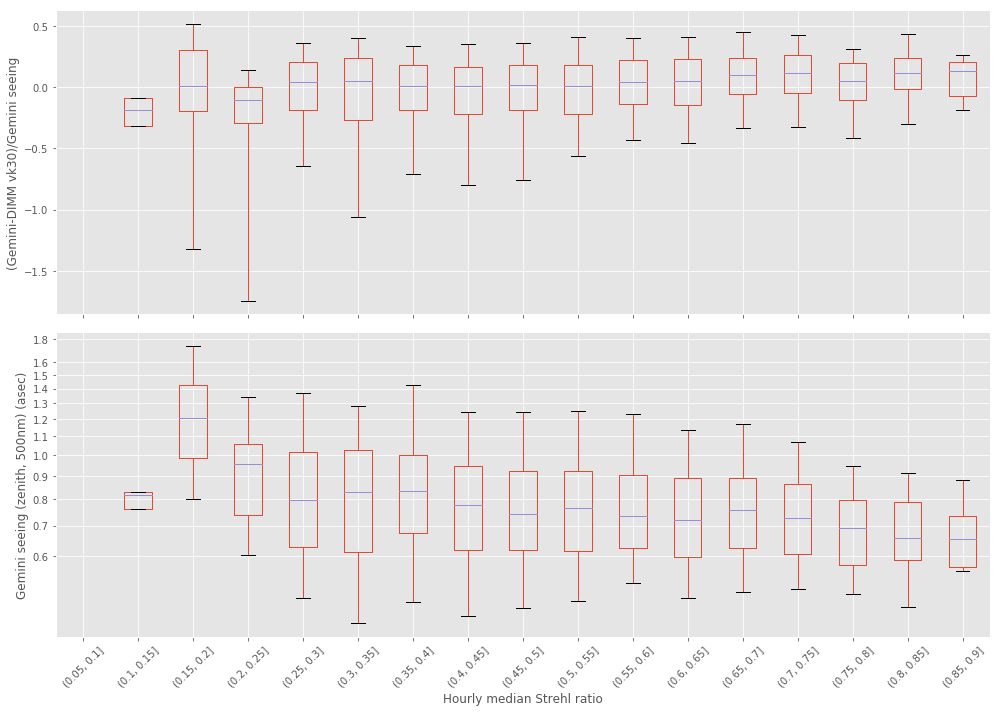
\includegraphics[width=\columnwidth]{./figures/gemini_strehl_boxplots.png}
  \caption{
    The upper panel shows the distribution of the fractional
    difference between DECam and DIMM seeing in hourly bins, split by
    the median DIMM Strehl ratio for these bins. The lower panel shows
    a similar distribution of the simple DECam seeing, similarly
    binned. Blue bars show the median, and red boxes the second and
    third quartiles. Whiskers indicate the 5\% and 95\% quantiles.
    }
  \label{fig:strehl-boxplots}
\end{figure*}

\begin{figure*}
  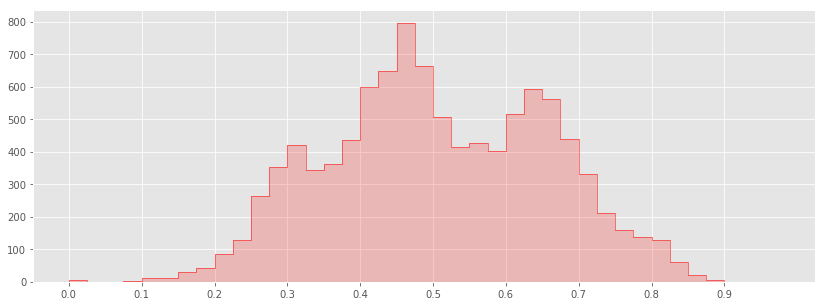
\includegraphics[width=\columnwidth]{./figures/strehl_hist.png}
  \caption{
    A histogram of the median Strehl ratio in each hour of DIMM observing.
  }
  \label{fig:strehl-hist}
\end{figure*}

\section{Generating a time series model for the DIMM data}

\subsection{The Fried parameter}

The best developed methodologies for modeling time series naturally
result in normal distributions: if we can transform the data set to be
modeled to roughly match a normal distribution, then a wider variety
of tools are available. The FWHM, as reported by the DIMM, has a
highly skewed distribution, with a long poor seeing tail, and a sharp
limit to the good seeing. One physically meaningful quantity that can
be mapped to the seeing is the Fried parameter, $r_{0}$: the diameter of a
circular aperture over which the RMS wavefront error induced by
atmospheric turbulence is one radian. This can be calculated for each
reported DIMM value by inverting equation~5 of
\cite{2002PASP..114.1156T}.  Figure~\ref{fig:r0-dist} shows the
distribution of measured values for the DIMM seeing (FWHM arcseconds)
and $\log(r_0)$ (right), together with best fit normal
distributions. Neither distribution is precisely normal, but $\log(
r_0)$ is noticeably closer.

\begin{figure*}
  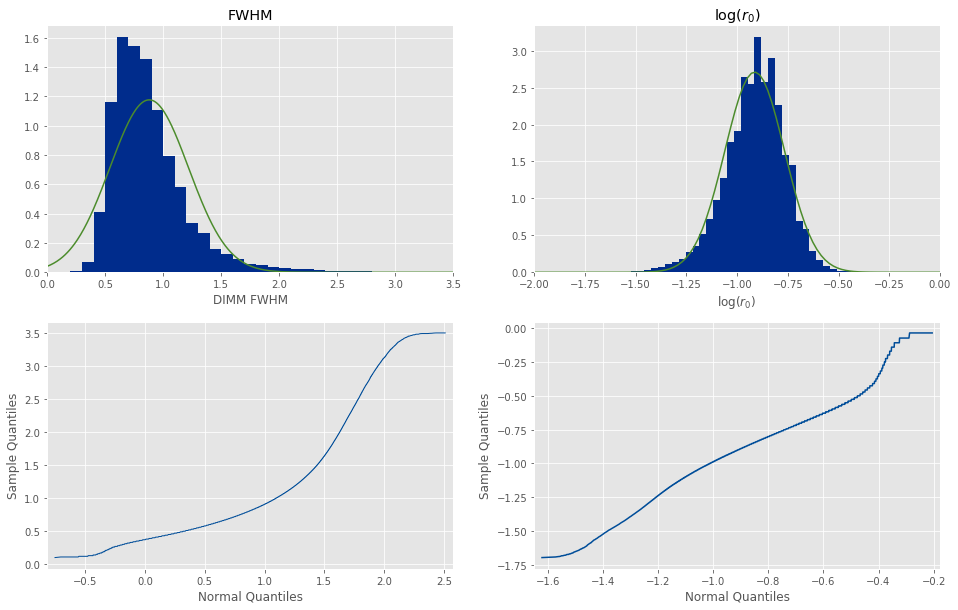
\includegraphics[width=\columnwidth]{./figures/r0_dist.png}
  \caption{The upper row shows the distribution of the DIMM seeing in
    arcseconds (left), and $\log(r_0)$ (right), together with best fit
    normal distributions. The lower row shows the corresponding
    probability plots. A straight line with a slop of one would
    indicate a perfect match between the data and the best fit normal
    distribution.}
  \label{fig:r0-dist}
\end{figure*}

%% The
%% nightly autocorrelation of the nightly mean values of $r_0$
%% (figure~\ref{fig:raw-dimm-autocorr}) also shows the seasonal effect.
%% \begin{figure*}
%%   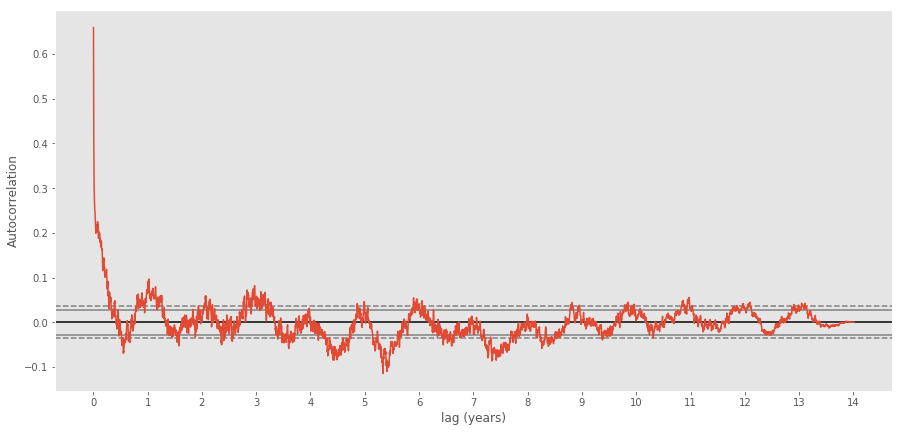
\includegraphics[width=\columnwidth]{raw_dimm_autocorr.png}
%%   \caption{The autocorrelation function of the mean values of $\log(
%%     r_0$. The horizontal solid and dashed bars mark the 95\% and 99\%
%%     confidence intervals for uncorrelated data.}
%%   \label{fig:raw-dimm-autotorr}
%% \end{figure*}


Figure~\ref{fig:random-nights-dimm} shows the time series of DIMM
measurements for three nights, chosen randomly from nights with
good DIMM coverage. 

\begin{figure*}
  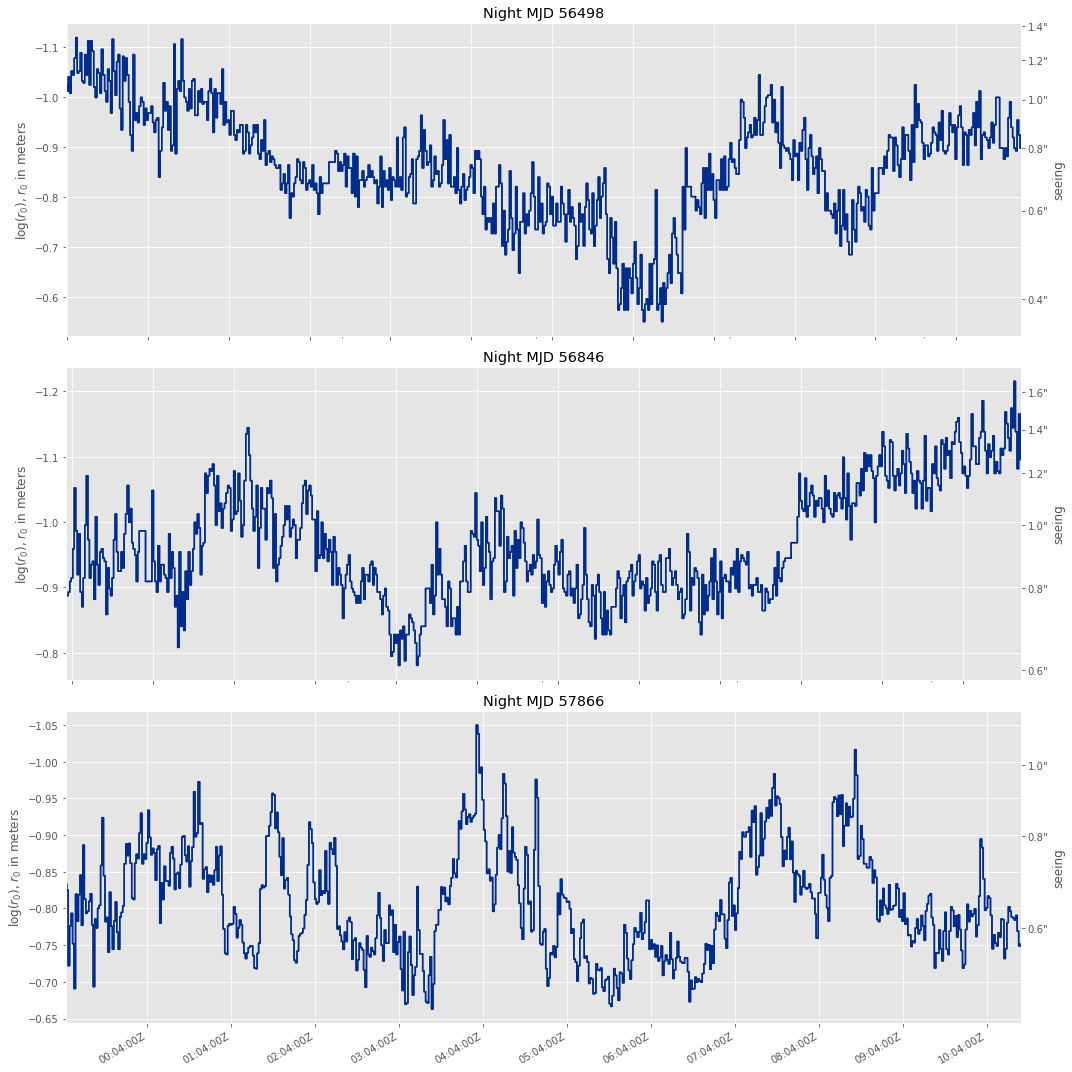
\includegraphics[width=\columnwidth]{./figures/random_nights_dimm.png}
  \caption{The time series of DIMM
measurements for three nights, chosen randomly from among nights with
good DIMM coverage. }
  \label{fig:random-nights-dimm}
\end{figure*}

\subsection{Seasonal fit}
\label{sec:seasonal}

The first stage in creating a model for the seeing data was to fit a
sine curve (plus a constant) with a period of one year to
$\log(r_0)$ (equation~\ref{eq:seasonal-sine}).

\begin{equation} \label{eq:seasonal-sine}
\log(r_0) = a + c \times \cos\left( (\mbox{day} - d) \times \frac{2\pi}{365.24217} \right)
\end{equation}

\begin{table}
\begin{center}
  \begin{tabular}{ l l l } \hline
      & uncut & cut \\ \hline
  $a$ & -0.9163 & -0.9119\\
  $c$ & 0.04 & 0.04 \\
  $d$ & 24.3 &  23.2 \\ \hline
  Nightly $\mbox{L1}$ & 0.23 & 0.22 \\
  Nightly $e$ & 0.082 & 0.088\\ \hline
  5 minute $\mbox{L1}$ & 0.68 & 0.73\\
  5 minute $e$ & 0.052 & 0.052\\ \hline
\end{tabular}
\caption{Parameters for the least squares fit of Pachon DIMM data to
  equation~\ref{eq:seasonal-sine}, the nightly autoregressive model,
  and the short time-scale autoregressive model.}\label{tab:fit-params}
\end{center}
\end{table}

A sine was chosen for its simplicity, and because the data did not
seem to support the use of a more complex
model. The first subsection of table~\ref{tab:fit-params} shows the best fit
values for the constants in equation~\ref{eq:seasonal-sine}. Figure~\ref{fig:monthly-boxplot} shows the distribution of the
mean $\log(r_0)$ values for each month, before and after subtraction
of the seasonal model. Before subtraction of the model, months near
the middle of the year have obviously worse seeing, an effect not
visible after subtraction. Figure~\ref{fig:seasonal-sub-autocorr}
shows the autocorrelation functions of the monthly mean $\log(r_0)$
values. The seasonal effect is again prominent before subtraction of
the seasonal fit. Longer timescale variations are still apparent after
subtraction of the seasonal model, but there is no obvious periodic
structure.

\begin{figure*}
  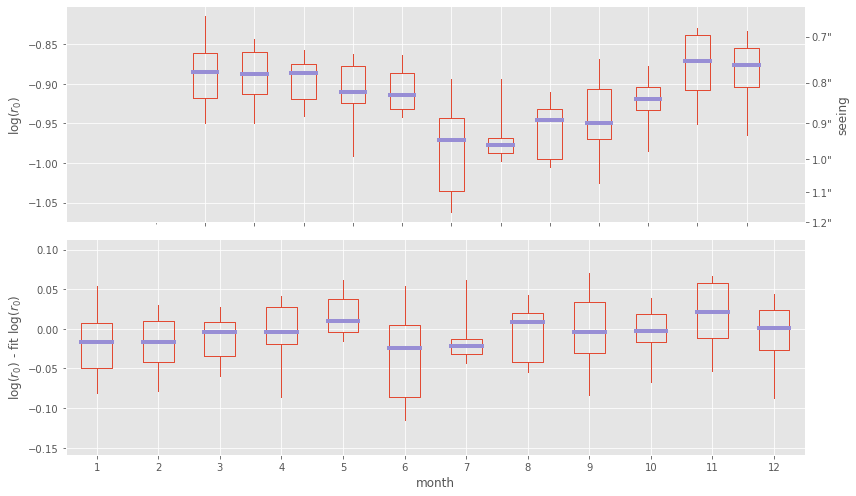
\includegraphics[width=\columnwidth]{./figures/monthly_boxplot.png}
  \caption{The top plot shows the distributions of mean monthly values
    for each month. The blue bar shows the median mean value for that
    month, the box the 1st and 3rd quartiles, and the whiskers the
    5\% and 95\% quantiles. The bottom plot shows the distributions after
    subtraction of the seasonal fit to $\log(r_0)$.}
  \label{fig:monthly-boxplot}
\end{figure*}

\begin{figure*}
  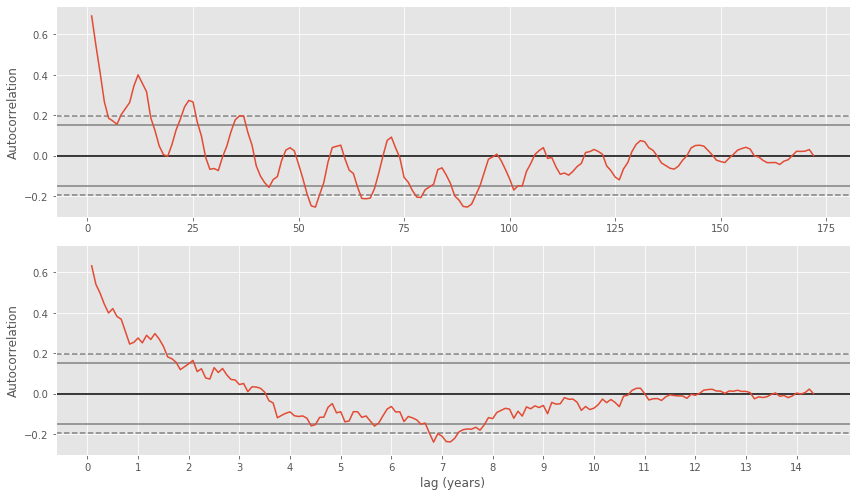
\includegraphics[width=\columnwidth]{./figures/seasonal_sub_autocorr.png}
  \caption{The upper and lower plots show the autocorrelation function
  of the mean $\log(r_0)$ by month, before and after subtraction of
  the seasonal model, respectively. The solid and dashed gray lines show
  the 95\% and 99\% ranges for uncorrelated data.}
  \label{fig:seasonal-sub-autocorr}
\end{figure*}

\subsection{Nightly variation in seeing}
\label{sec:nightly-variation}

After subtraction of the seasonal variation in $\log(r_0)$,
significant night to night correlation remains. These are modeled here as a
first-order autoregressive process [\cite{cryer_time_2008}], also
referred to as an AR(1) process\footnote{An AR(1) processes is equivalent to a damped random walk
[\cite{2009ApJ...698..895K}]}, described in
equation~\ref{eq:ar1}. $y_t$ is the difference between the mean
$\log(r_0)$ on that night and the seasonal model for
$\log(r_0)$. $\mbox{L1}$ is the regressive term, the model parameter
that represents the correlation between one night and the next, and
$e_t$ is the ``innovation'', analogous to the step sizes in a random
walk.

\begin{equation} \label{eq:ar1}
y_t = \mbox{L1} \times y_{t-1} + e_t
\end{equation}

There are many nights in the Cerro Pachon DIMM data set with no data.
The tool used to fit the AR1 model, from the python
\texttt{statsmodels} module [\cite{seabold2010statsmodels}], does not
handle missing data. To fit the AR1 model, I divided the full data set
into sequences of consecutive nights without missing data, performed
separate fits on each sequence, and accepted the mean values provided
by the models, weighted according to the reported uncertainty in each
model fit. Table~\ref{tab:fit-params} lists the resultant fit
parameters.

The distribution values in a sequence of points generated by an AR1
process is a normal distribution with a variance given by
equation~\ref{eq:ar1var}[\cite{cryer_time_2008} eqn. 4.3.3].

\begin{equation} \label{eq:ar1var}
\sigma_y^2 = \frac{\sigma_e^2}{1-\mbox{L1}^2}
\end{equation}

Figure~\ref{fig:night-ar1-dist} shows the expected distribution given
the fit model parameters over-plotted over the actual histogram of
$\log(r_0)$ - seasonal fit $\log(r_0)$. The distribution expected from
the AR1 fit is sharper than the measured one, and does not capture the
tail on the low-$\log(r_0)$ side of the distribution. The latter is a
fundamental limitation of the model. The sharper distribution likely
arises from the fit of a collection of sub-sequences of nights, rather
than a full, uninterrupted data set:
figure~\ref{fig:decam-monthly-dimm-vs-year} clearly shows variations on
timescales of months to years, too long to be captured by the
sub-sequences of nights to which the AR1 model was fit.

\begin{figure*}
  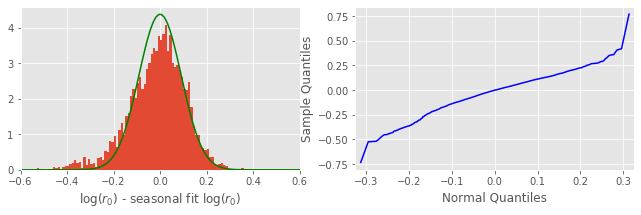
\includegraphics[width=\columnwidth]{./figures/night_ar1_dist.png}
  \caption{The histogram of differences between nightly mean
    $\log(r_0)$ and the seasonal fit, over-plotted by the result that
    would be expected by the fit AR1 model.}
  \label{fig:night-ar1-dist}
\end{figure*}

\subsection{Short timescale variation in seeing}
\label{sec:short-variation}

In addition to varying on a nightly basis, seeing varies on much
shorter timescales. The short-timescale variations are modeled using
an AR1 model as well. The raw DIMM data is sampled irregularly,
slightly more frequently than once every 5 minutes. I therefore
resample the points onto exact 5-minute intervals, and divide it in into
sub-sequences of consecutive uninterrupted exposures, similar to the
procedure for nightly data. Table~\ref{tab:fit-params} lists the
resultant fit parameters.

\subsection{Correction from Kolmogorov to von K\'arm\'an turbulence}
\label{sec:vkcorr}

The raw data provided by the Cerro Pachon DIMM archive provides seeing
data calculated using a Kolmogorov model for the turbulence in the
atmosphere. This data was used to work backward to the Fried
parameter, $r_0$, which was then modeled. To obtain simulation seeing
values from the $r_0$ model, I use the approximation given in
equation~\ref{eq:ktovk}, provided by \cite{2002PASP..114.1156T}.

\begin{equation} \label{eq:ktovk}
\left( \frac{\mbox{FWHM}_{vK}}{\mbox{FWHM}_{K}} \right)^2
\approx 1 - 2.183 \left( \frac{r_0}{\mathcal{L}_0} \right)^{0.356}
\end{equation}

I use a value of $\mathcal{L}_0 = 30$ meters, based on the
value of $28.4^{+25.0}_{-13.3}$ meters reported by
\cite{2000ApOpt..39.5415Z} for Cerro Pachon. This corresponds to a 22\%
improvement in seeing when converting from a Kolmogorov to a
von~K\'arm\'an turbulence model and a typical value of $r_0$, but the
range given is from 18\% to 30\%. Furthermore, the value reported was
measured data from only a few nights of data, and is likely to be
strongly dependent on weather.

\subsection{Seeing data generation}
\label{sec:data-generation}

Much of the data to be used by an \texttt{opsim} simulation can be copied
directly from the historical DIMM data, after conversion from a
Kolmogorov to a von~K\'arm\'an turbulence model and application of an
offset in time by an integer number of years. The gaps can then be
filled in using the model.

For sequences of nights with no data, mean values for each night are
calculated using the seasonal model (equation~\ref{eq:seasonal-sine})
and the nightly AR1 model (equation~\ref{eq:ar1}) with the last night
of data with DIMM data and randomly generated values of $e_t$. For
sequences of short time-scale (5 minute interval) points, artificial
data is generated similarly, using the nightly mean, the last good
DIMM data point, and random values of $e_t$.

Two different seeing databases were generated: one using a 13 year
offset (such that the 2022-01-01T00:00:00Z data point in the data set
is copied from the 2009-01-01T00:00:00Z DIMM data), and one using a 16
year offset, such that we take full advantage of all available DIMM
data. Note that there is overlap between the DIMM data used by these
two database, so the results are not uncorrelated.

\section{\texttt{opsim} simulations}
\label{sec:simulations}

Three separate simulations were run using \texttt{opsim}, specifically
\texttt{sims\_featureScheduler} revision \texttt{b9f8585} and
\texttt{sims\_featureScheduler\_runs\_1.3} revision
\texttt{2aba222}. Each simulation was run for a full 10-year LSST
survey, with the default configuration except for the seeing database.

\begin{description}
   \item[{\tt baseline\_v1.3\_10yrs}] a 10-year simulation using the defaults
     seeing database, used as a reference.
  \item[{\tt ss58777y13\_v1.3\_10yrs}] a simulation using the
    {\tt simsee\_pachon\_58777\_13.db} seeing database, which uses
    uncut DIMM data from 2009-01-01 to 2019-10-07 to simulate
    2022-01-01 to 2033-10-07 and the seeing model derived from uncut
    DIMM data to generate simulated data for gaps. This simulation is otherwise identical
    to {\tt baseline\_v1.3\_10yr}.
  \item[{\tt ss58777y16\_v1.3\_10yrs}] a simulation using the
    {\tt simsee\_pachon\_58777\_16.db} seeing database, which uses
    uncut DIMM data from 2006-01-01 to 2019-10-07 to simulate
    2022-01-01 to 2036-10-07 and the seeing model derived from uncut
    DIMM data to generate simulated data for gaps. This simulation is otherwise identical
    to {\tt baseline\_v1.3\_10yr}.
  \item[{\tt ss58779y13\_v1.3\_10yrs}] a simulation using the
    {\tt simsee\_pachon\_58779\_13.db} seeing database, which uses
    cut DIMM data from 2009-01-01 to 2019-10-07 to simulate 2022-01-01
    to 2033-10-07 and the seeing model derived from cut DIMM data to
    generate simulated data for gaps. This simulation is otherwise
    identical to {\tt baseline\_v1.3\_10yr}.
  \item[{\tt ss58779y16\_v1.3\_10yrs}] a simulation using the
    {\tt simsee\_pachon\_58779\_16.db} seeing database, which uses
    cut DIMM data from 2006-01-01 to 2019-10-07 to simulate 2022-01-01
    to 2036-10-07 and the seeing model derived from cut DIMM data to
    generate simulated data for gaps. This simulation is otherwise
    identical to {\tt baseline\_v1.3\_10yr}.
\end{description}

Figure~\ref{fig:simseecomp} shows the seeing as a function of time, as
recorded in the databases produced by each of the five runs of
\texttt{opsim}. The two year periodicity of the seeing that results
from the default two year input database is apparent in the leftmost
plot in the figure. Yearly periodicity, expected from the seasonal
variation in the DIMM data and model, is apparent in the plots from
the other two runs. 


\begin{figure*}
\begin{center}
  \minipage{0.5\textwidth}
  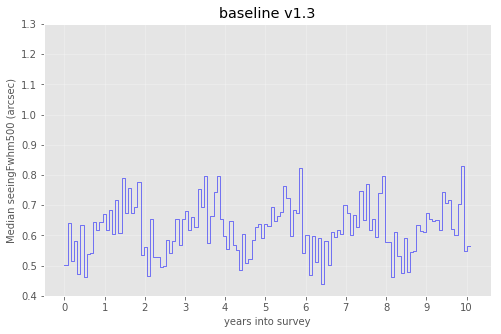
\includegraphics[width=\columnwidth]{./figures/seeing_baseline_v1_3_10yrs.png}
\endminipage\hfill
\end{center}
\minipage{0.5\textwidth}
  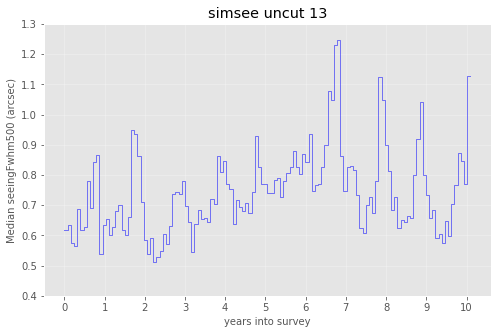
\includegraphics[width=\columnwidth]{./figures/seeing_ss58777y13_v1_3_10yrs.png}
\endminipage\hfill
\minipage{0.5\textwidth}
  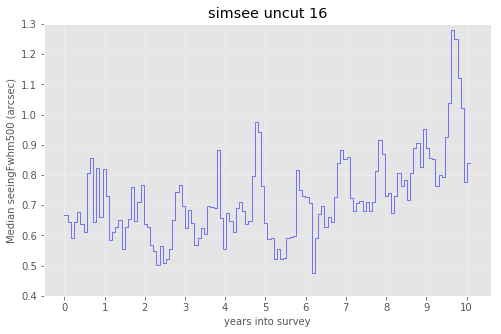
\includegraphics[width=\columnwidth]{./figures/seeing_ss58777y16_v1_3_10yrs.png}
\endminipage\hfill
\minipage{0.5\textwidth}
  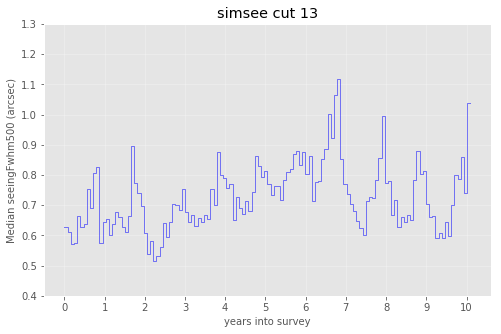
\includegraphics[width=\columnwidth]{./figures/seeing_ss58779y13_v1_3_10yrs.png}
\endminipage\hfill
\minipage{0.5\textwidth}
  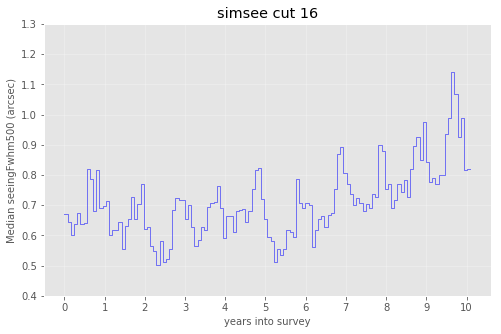
\includegraphics[width=\columnwidth]{./figures/seeing_ss58779y16_v1_3_10yrs.png}
\endminipage\hfill
  \caption{Each plot shows the variation in seeing with time
    produced by a different run of \texttt{opsim}. The top plot
    shows the seeing for the default seeing database, and the
    remaining plots show the seeing for each of the seeing databases
    produced by \texttt{simsee}.} 
  \label{fig:simseecomp}
\end{figure*}

Figure~\ref{fig:simseemaps} shows maps of the mean seeing in the LSST
wide-fast-deep (WFD) survey from each simulation. Degradation is
apparent near the northern and southern edges of all three
simulations. This is expected, because these areas are never at low
airmass from Cerro Pachon. At a give range in declination, there is
also variation with R.A. This variation is much more pronounced in the
revised seeing databases than in the baseline: in the baseline, the
best 6 hours of R.A. have a mean seeing 6\% better than the worst 6
hours, while for the revised seeing simulations, the difference is
about 12\% (or 14\% if no cut on Strehl ratio is applied). 

\begin{figure*}
\begin{center}
\minipage{0.5\textwidth}
  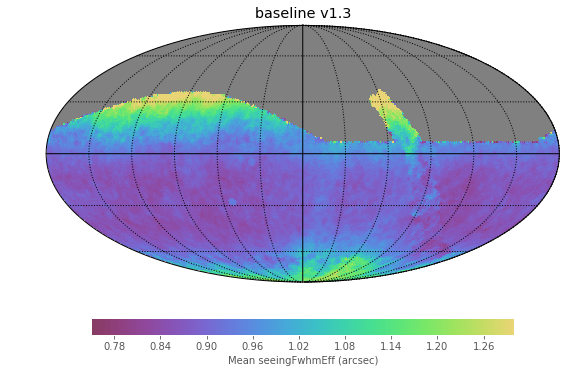
\includegraphics[width=\columnwidth]{./figures/seeing_map_baseline_v1_3_10yrs.png}
\endminipage\hfill
\end{center}
\minipage{0.5\textwidth}
  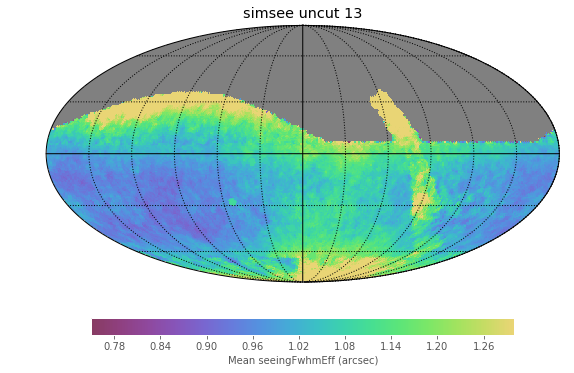
\includegraphics[width=\columnwidth]{./figures/seeing_map_ss58777y13_v1_3_10yrs.png}
\endminipage\hfill
\minipage{0.5\textwidth}
  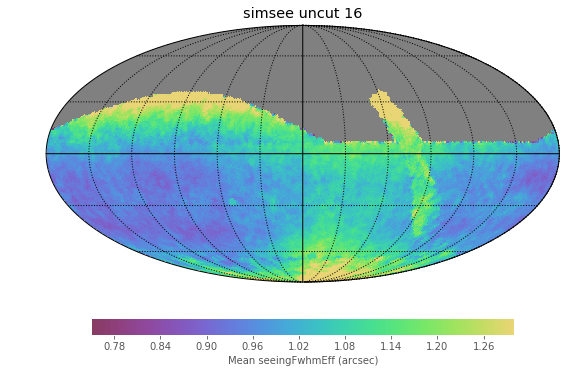
\includegraphics[width=\columnwidth]{./figures/seeing_map_ss58777y16_v1_3_10yrs.png}
\endminipage\hfill
\minipage{0.5\textwidth}
  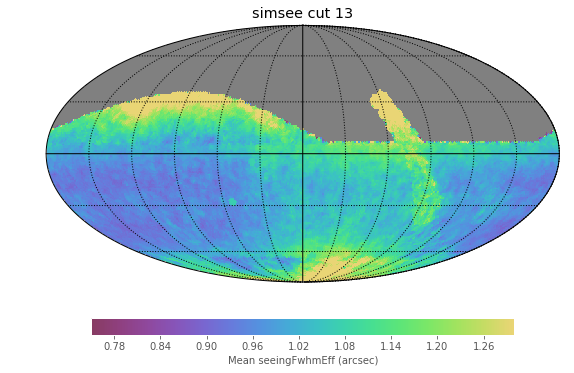
\includegraphics[width=\columnwidth]{./figures/seeing_map_ss58779y13_v1_3_10yrs.png}
\endminipage\hfill
\minipage{0.5\textwidth}
  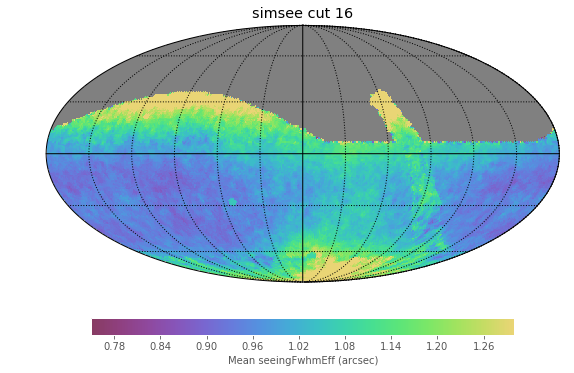
\includegraphics[width=\columnwidth]{./figures/seeing_map_ss58779y16_v1_3_10yrs.png}
\endminipage\hfill
  \caption{Each plot shows the map of mean seeing
    produced by a different run of \texttt{opsim}. The top plot
    shows the seeing for the default seeing database, and the
    remaining plots show the seeing for each of the seeing databases
    produced by \texttt{simsee}.} 
  \label{fig:simseemaps}
\end{figure*}

The variation in seeing corresponds to a variation in depth, shown in
figure~\ref{fig:simdepthmaps} and the right-hand plot in
figure~\ref{fig:seelimra}, so there is a
similar difference in the amplitude of variation for limiting
magnitude: in the baseline, there is a difference of about 0.14
magnitudes between the mean limiting magnitudes of the best and worst
6 hours of R.A., while in the revised seeing simulations the difference is
about 0.20 magnitudes.

\begin{figure*}
\begin{center}
\minipage{0.5\textwidth}
  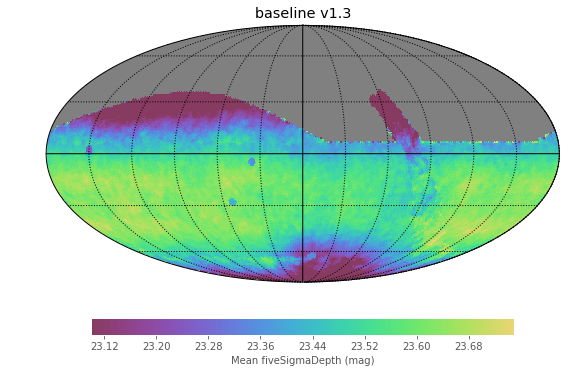
\includegraphics[width=\columnwidth]{./figures/depth_map_baseline_v1_3_10yrs.png}
\endminipage\hfill
\end{center}
\minipage{0.5\textwidth}
  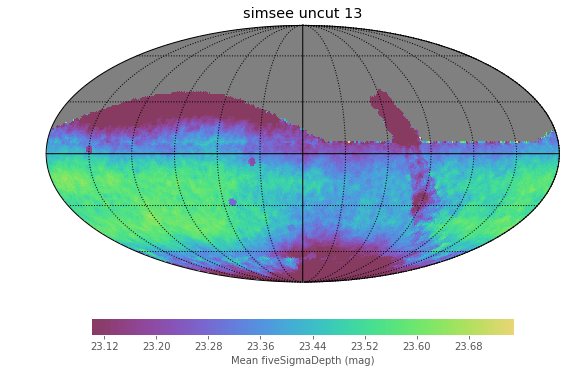
\includegraphics[width=\columnwidth]{./figures/depth_map_ss58777y13_v1_3_10yrs.png}
\endminipage\hfill
\minipage{0.5\textwidth}
  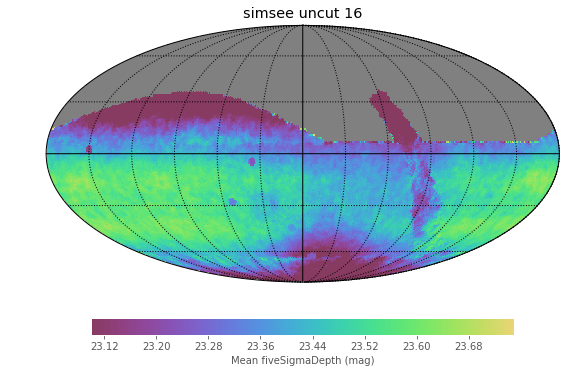
\includegraphics[width=\columnwidth]{./figures/depth_map_ss58777y16_v1_3_10yrs.png}
\endminipage\hfill
\minipage{0.5\textwidth}
  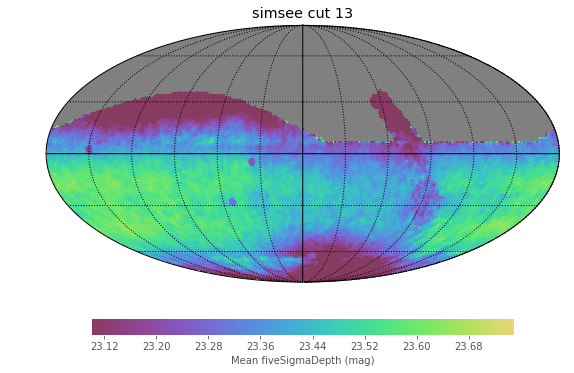
\includegraphics[width=\columnwidth]{./figures/depth_map_ss58779y13_v1_3_10yrs.png}
\endminipage\hfill
\minipage{0.5\textwidth}
  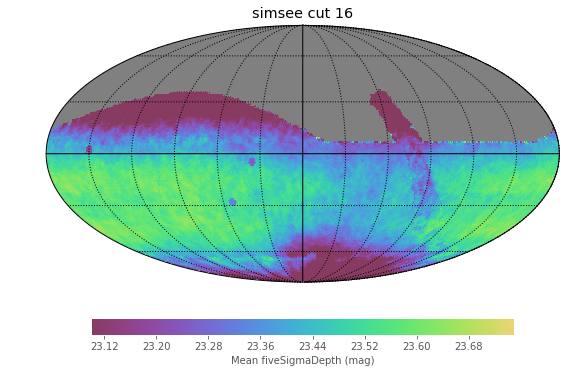
\includegraphics[width=\columnwidth]{./figures/depth_map_ss58779y16_v1_3_10yrs.png}
\endminipage\hfill
  \caption{Each plot shows the map of mean depth
    produced by a different run of \texttt{opsim}. The top plot
    shows the depth for the default seeing database, and the
    remaining plots show the depth for each of the seeing databases
    produced by \texttt{simsee}.} 
  \label{fig:simdepthmaps}
\end{figure*}

\begin{figure*}
  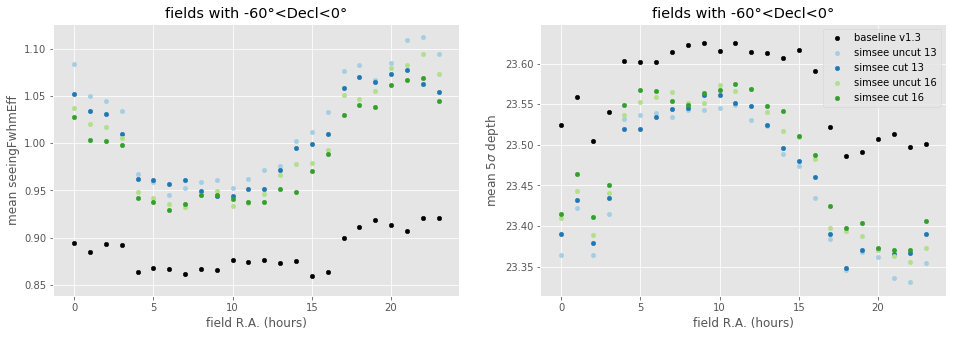
\includegraphics[width=\columnwidth]{./figures/seeing_depth_by_ra.png}
  \caption{The seeing and depth as a function of RA for different runs
  of \texttt{opsim4}.} 
  \label{fig:seelimra}
\end{figure*}

\begin{table}
\begin{center}
\begin{tabular}{lrrrrrrrrrrrr}
\hline
{} & \multicolumn{6}{l}{mean} & \multicolumn{6}{l}{IQR} \\
band &     g &     i &     r &     u &     y &     z &     g &     i &     r &     u &     y &     z \\
simulation      &       &       &       &       &       &       &       &       &       &       &       &       \\
\hline
baseline v1.3   &  1.00 &  0.91 &  0.94 &  1.07 &  0.87 &  0.90 &  0.31 &  0.26 &  0.28 &  0.35 &  0.23 &  0.25 \\
simsee cut 13   &  1.14 &  1.03 &  1.07 &  1.20 &  0.99 &  1.01 &  0.39 &  0.33 &  0.35 &  0.41 &  0.32 &  0.32 \\
simsee cut 16   &  1.13 &  1.01 &  1.05 &  1.21 &  0.98 &  0.99 &  0.39 &  0.33 &  0.36 &  0.43 &  0.31 &  0.32 \\
simsee uncut 13 &  1.16 &  1.05 &  1.09 &  1.24 &  1.00 &  1.03 &  0.40 &  0.34 &  0.37 &  0.44 &  0.33 &  0.34 \\
simsee uncut 16 &  1.13 &  1.02 &  1.06 &  1.23 &  0.98 &  1.00 &  0.41 &  0.34 &  0.37 &  0.43 &  0.31 &  0.32 \\
\hline
\end{tabular}
\caption{The mean and inter-quartile range of the FWHM in opsim
  simulations, by filter, for the baseline and each replacement seeing
  simulation.}\label{tab:sim-stats}
\end{center}
\end{table}

Table~\ref{tab:sim-stats} lists the mean and inter-quartile range (IQR) of the seeing in images from each simulation, showing the consequences of the change in seeing database for both the average seeing and its uniformity in the v1.3 simulations.

% ----------------------------------------------------------------------

\section{Discussion}
\label{sec:discussion}

The use of a longer baseline of real seeing data (and a more elaborate
model for times when such data is not available) in operations
simulations demonstrates a significant, large angular scale variation
in seeing (and therefore depth) using the current strategy, as well as
a mean shift to wider PSF (and therefore shallower limiting
magnitude). The impact of this variation on science results needs to
be carefully evaluated and, if warranted by the science, adjustments
to the strategy made to mitigate these effects.

Such mitigation strategies will necessarily come at a cost. The
current strategy is designed to observe fields when they are near
transit. Such a strategy optimizes the quality of data taken at any
given time: a field observed near transit at a given declination will
have a better FWHM than another at the same declination, but further
from transit. Observing fields near transit, however, necessarily maps
time of observation directly to sidereal time, which is correlated
with time of year, and therefore the seasonal variation in seeing.

This correlation can be reduced by observing fields when they are
further from transit, depending on seeing conditions. Such a strategy
can be designed to even out the extremes in the variation. However, if
the strategy maintains the global distribution in declination, these
exposures will be at higher airmasses than those that would have been
taken at transit. This will degrade the overall mean image quality.

A compromise will need to be made. The effect on image quality is not
linear with zenith distance (or time from transit), but is shallow
very close to transit, and degrades more rapidly as the angle
increases: a mild deviation from the transiting strategy may only have
a mild effect on the mean image quality.

\section{Future work}
\label{sec:future}

Although an improvement over the default seeing database, the revised
seeing databases presented here leave significant room for
improvement. Some refinements that could be explored include:

\begin{itemize}

\item Creating a better model of the poor seeing tail in the
  distribution of seeing values, either as an additional component or
  by transforming the DIMM's $\log(r_0)$ distribution.

\item Interactive exploration and informal experience suggest that the
  seeing has a systematic variation with the time of night, in
  particular that the seeing is slightly worse shortly after
  sunset. This needs to be studied further, and perhaps modeled as
  well.

\item Rigorous evaluation of higher-order ARMA models using a formal
  criteria (either Akaike's Information Criterion (AIC) or a Bayesian
  Information Criterion (BIC))[\cite{cryer_time_2008} pp. 130-132],
  rather than the AR1 model used here. The AR1 model was selected due
  to its simplicity and apparent effectiveness after informal
  exploration; additional terms and/or a moving average component may
  be warranted.

\item Modeling the short term, nightly, seasonal, and long-term
  components as a single seasonal ARMA model, following the formalism
  described in \cite{cryer_time_2008} chapter 10. Rather than fit each
  element separately (as has been done here), this approach
  incorporates long-term effects by including additional terms in the
  autoregressive equation.
  
\item Modeling using a continuous ARMA model (CARMA)
  [\cite{brockwell_introduction_1996} pp. 344-348] rather than the
  discrete ARMA model used here. Such models are significantly more
  complex and lack the well developed software tools, but naturally
  handle the irregularly sampled nature of the DIMM data.
  
\end{itemize}

Long term (multi-year) trends in seeing are apparent in the DIMM data,
however, and improvement from any of the above seems likely to be
minor compared to the uncertainty due to these trends. Finally, it
seems unlikely that any of these improvements will have a major effect
on survey strategy metrics anyway.

In addition to modeling the seeing, improved modeling of the effect of
clouds in survey data quality should also be studied.

% ----------------------------------------------------------------------

\section{Conclusion}
\label{sec:conclusion}

The full archive of data from the Cerro Tololo DIMM shows strong
seasonal variations, and larger mean values for the seeing, than are
present in the default input database used by the LSST \texttt{opsim}
operations simulator. Inclusion of an updated seeing database is
therefore important for using \texttt{opsim} to evaluate both the
overall survey quality and also large-scale variation in seeing and
depth across the survey footprint.

% ----------------------------------------------------------------------

\subsection*{Acknowledgments}

I am grateful to Edison Bustos and other staff of the National Optical
Astronomical Observatory (NOAO) for supplying the data used in this
study, and discussions with Chuck Claver that led to an understanding
of the origin of the baseline data set.

This manuscript has been authored by Fermi Research Alliance, LLC
under Contract No. DE-AC02-07CH11359 with the U.S. Department of
Energy, Office of Science, Office of High Energy Physics.



\appendix
% Include all the relevant bib files.
% https://lsst-texmf.lsst.io/lsstdoc.html#bibliographies
\section{References} \label{sec:bib}
\renewcommand{\refname}{} % Suppress default Bibliography section
\bibliography{local,lsst,lsst-dm,refs_ads,refs,books}

% Make sure lsst-texmf/bin/generateAcronyms.py is in your path
\section{Acronyms} \label{sec:acronyms}
\addtocounter{table}{-1}
\begin{longtable}{p{0.145\textwidth}p{0.8\textwidth}}\hline
\textbf{Acronym} & \textbf{Description}  \\\hline

2D & Two-dimensional \\\hline
DE & dark energy \\\hline
DES & Dark Energy Survey \\\hline
DIMM & Differential Image Motion Monitor \\\hline
DM & Data Management \\\hline
FWHM & Full Width at Half-Maximum \\\hline
L1 & Lens 1 \\\hline
LSST & Legacy Survey of Space and Time (formerly Large Synoptic Survey Telescope) \\\hline
MJD & Modified Julian Date (to be avoided; see also JD) \\\hline
NOAO & National Optical Astronomy Observatories (USA) \\\hline
PSF & Point Spread Function \\\hline
RA & Right Ascension \\\hline
RMS & Root-Mean-Square \\\hline
RTN & Rubin Technical Note \\\hline
WFD & Wide Fast Deep \\\hline
\end{longtable}

% If you want glossary uncomment below -- comment out the two lines above
%\printglossaries





\end{document}
